\documentclass[12pt]{article}
\usepackage{color}
\usepackage[usenames,dvipsnames,svgnames,table]{xcolor}
\definecolor{dark-red}{rgb}{0.7,0.1,0.1} 
\definecolor{dark-blue}{rgb}{0,0,0.7} 
\usepackage[linkcolor=dark-red,
            colorlinks=true,
            urlcolor=dark-blue,
            pdfstartview={XYZ null null 1.00},
            pdfauthor={Gaurav Sood, gsood07@gmail.com},
            citecolor=dark-red,
            bookmarks=false,
            pdfborder={0 0 0},
            pdftitle={Fairly Random}]{hyperref}
            
\usepackage{amsfonts,amssymb,amsbsy,amsmath,amsxtra}

\usepackage[letterspace=1000]{microtype}
\usepackage{libertine}
\usepackage[T1]{fontenc}

\usepackage{indentfirst}
\usepackage{setspace} % To set line spacing
\usepackage{multirow}

\usepackage{verbatim}

\usepackage[multiple]{footmisc}
\usepackage{fancyvrb}

\usepackage{longtable}

\usepackage[margin=1in]{geometry}
\usepackage{graphicx}

\raggedright
\parindent=1.5em % <- or whatever indent you want

\usepackage{natbib}
\usepackage{url}
\begin{comment}

setwd(paste0(githubdir, "/cricket-stats/write_up/"))	
tools::texi2dvi("cricket.tex", pdf=TRUE, clean=TRUE)	
setwd(paste0(githubdir, "/cricket-stats/"))

\end{comment}

\begin{document}
\title{\vspace{-.5cm}\normalsize{Fairly Random: Impact of Winning the Toss on the Probability of Winning\footnote{You can find the scripts used to scrape the data, the final data set, and scripts used for analysis at: \href{https://github.com/dwillis/cricket-stats}{https://github.com/dwillis/cricket-stats}.}\vspace{.5cm}}}
\author{\normalsize{Gaurav Sood}\\\href{mailto:gsood07@gmail.com}{\small{gsood07@gmail.com}} \and \normalsize{Derek Willis}\\\href{mailto:dwillis@gmail.com}{\small{dwillis@gmail.com}}}
\date{\vspace{.5cm}\normalsize{\today}}
\maketitle
\doublespacing

In nearly all cricket matches, it is claimed that there is a clear advantage to either bowling or batting first. The advantage is pointed to by commentators, by the team captains in the pre-toss interview, and by the captain of the losing team in the post-match interview. And to wrest the said advantage, the captain merely needs to pick the side of the coin that will be left facing the sky after the toss. And while this method of granting advantage is fair on average, the system isn't fair in any one game. 

At first glance, this imbalance seems inevitable. After all, someone has to bat first. One can, however, devise a baseball like system, with a series of short innings woven together. If that violates the nature of the game too much, one can easily create pitches that don't deteriorate appreciably over the course of a match. Or, one can come up with an estimate of the advantage, and adjust the scores accordingly, akin to an adjustment that is issued when the matches are shortened due to rain.

None of this to say that there is actually an advantage in winning the toss, or that teams are able to successfully exploit any such advantage. For it may be impossible to predict well in advance the advantage of bowling or batting first. Or, it may be that teams squander the potential advantage by using bad heuristics to choose what they do. 

To assess the net observed advantage of winning the toss, we exploit data from a novel dataset of over 43,000 first-class men's cricket matches --- to our knowledge, the largest ever dataset assembled for the question, and nearly 50--100 times larger than used in prominent previous attempts \citep[see,][]{dawson2009bat, de1998winning}. In analyzing these data, we avoid a common but important pitfall that some other studies on the topic fall into. To avoid post-treatment bias \citep[see][]{acharya2015}, unlike \citet{dawson2009bat}, \citet{Saad2015}, etc., we do not condition on post coin-toss decisions. We find that winning the toss grants a small but significant advantage, but that advantage varies considerably and systematically. 

\section*{Data}
Data are from 43,185 first-class men's cricket matches. It is a near census of the relevant population. We have data on all types of matches: domestic and international Twenty20s --- T20s and T20Is respectively, domestic and international one-dayers --- List A and One-Day Internationals (ODI) respectively, and domestic and international multi-day matches --- First Class (FC) and Tests respectively.\footnote{There is a rich variety of first-class matches. In English county cricket, first-class matches last four days. Some first class matches last just a day. Others two days. Yet others three days. And till a particular point in history, a test match lasted as long as it was needed to finish a game. We elide over such differences.} 

Of these matches, we do not have data on the toss for 2,807, or roughly 7\%, of the matches. The primary reason we don't have data on these matches is because the match was abandoned without play. We exclude data from these matches. 

In limited overs cricket, a minimum number of overs must be bowled to establish a result. In a one-day match, for instance, each side must bat at least 20 overs for a result to be declared. In 706 matches, or roughly 1.7\% of the remaining matches, not enough overs were bowled to get a result. We again exclude these matches from our analysis. This leaves us with 39,672 matches. We analyze these data.
 
\section*{Analyses and Results}

We assume that the outcome of a toss is random. Conditional on the outcome of a toss being random, the effect of winning the toss can be attributed to the toss itself. Any decision made after the outcome of the toss is known, however, is `post-treatment.' In particular, the decision to bat or bowl first is made after accounting for the relative strengths and weaknesses vis-\`{a}-vis the competing team at that particular instance, and thus not independent of team attributes. Hence, conditioning on decision to bowl or bat first can induce bias in estimates of advantage of winning a toss. Thus, unlike \citet{dawson2009bat}, \citet{Saad2015}, we solely rely on the assumption that the outcome of a toss is random. 

But before we exploit the design, we shed some light on the validity of the assumption. In particular, we assess whether the coin toss is somehow rigged, with the home side enjoying the rub of the green more often. For this analysis, we only get to exploit international matches as establishing which of the teams is the home team in local matches is somewhat arduous. Of the 5,591 international matches, the home team won the toss in 2,860 matches, or about 51.15\%. The probability that we will get as large a proportion by chance after tossing 5,591 coins is about 8.7\%, low but not eyebrow-raisingly so. Thus, for now, we choose to trust that the tosses are random.

A caveat about interpretation before we report the results. As we discuss in the introduction, we cannot estimate the actual advantage of winning a toss. We can only estimate the net observed advantage, which is the extent to which the teams capitalize on the potential advantage. With that, the results.

The team that wins the toss wins the match 2.9\% more often than the team that loses the toss. This is a reasonable sized advantage in a competitive sport --- though likely much smaller than the number that most commentators carry in their heads.
% Also interpret it by comparing to probability of winning when playing with the worst placed team (not defined from last team)
This advantage, however, varies by format, by conditions, by whether or not a particular formula was used to adjust scores when it rains, and how much better the team that won the toss is vis-\`{a}-vis the competing team. Much of the variability follows expected patterns.

The conventional wisdom among lay cricket followers is that toss grants the greatest advantage in multi-day affairs like tests and first class matches, followed by day long affairs, and Twenty20s. And there is good dose of common sense behind the conventional wisdom. Pitches invariably deteriorate over multiple days and batting last in a test match is often the most challenging time to bat. The pitch deteriorates far less over the course of the day, or in case of Twenty20s, a few hours. And indeed unlimited over matches provide the most consistent advantage --- the average advantage over FC and test matches is north of 2.7\% (see Figure~\ref{fig:type}). Looked in relative terms, the advantage of winning the toss is also close to the greatest in multi-day affairs. Only about 60\% of test matches end in a  clear decision, the rest end in a draw. Thus, the advantage is closer to 4.5\%. 

The heftiest advantage, however, is in domestic one-day matches (List A), approximately 4.8\%. The number for ODIs, however, is a bit puzzling --- there is an advantage to winning the toss but it is really slight (.83\%). That can best be ascribed to choosing badly. In T20s and T20Is, the advantage is 1.3\% and 3.8\% respectively.      

\begin{figure}[htbp]
\caption{Difference in Winning Percentages of Teams that Won the Toss and Teams that Lost the Toss by Type of Match.}
\begin{minipage}{0.85\textwidth}
\centering
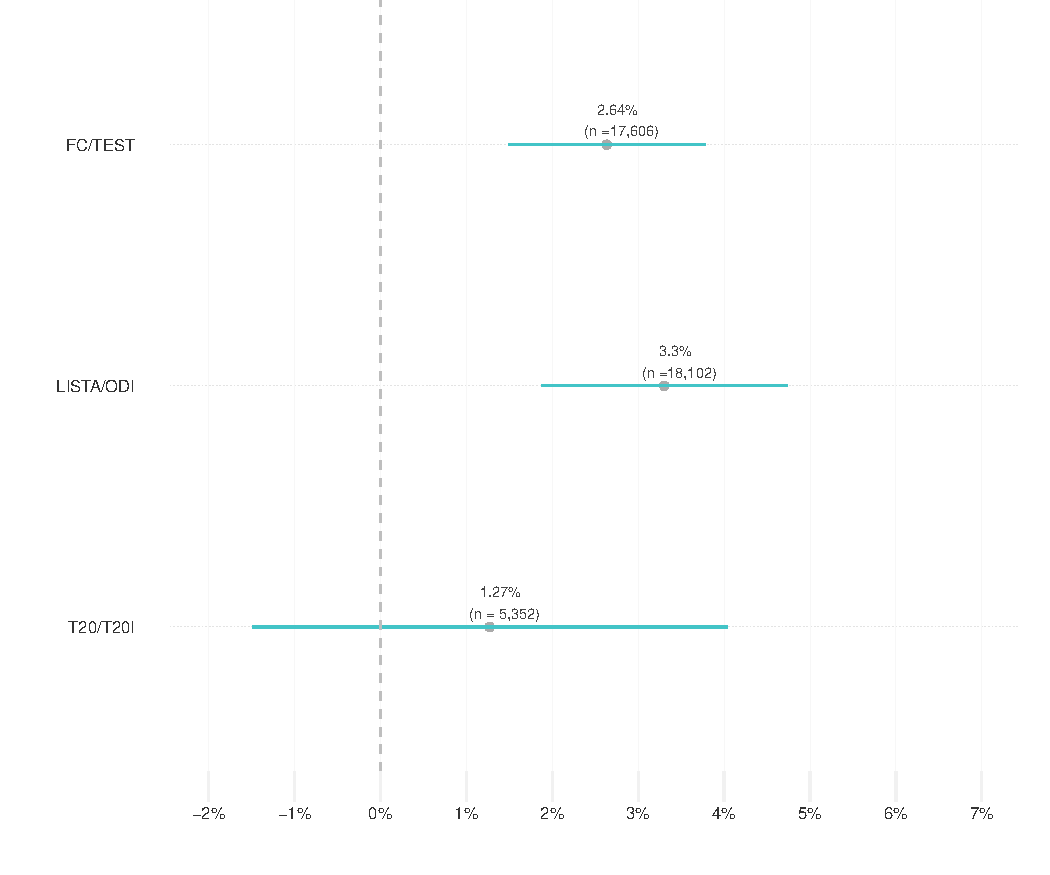
\includegraphics[scale=.85]{../figs/winbyType.pdf}
{\footnotesize Note: \emph{n} refers to the number of matches.\par}
\end{minipage}
\label{fig:type}
\end{figure}

But type of matches cover only major source of variation and theorizing about the advantage granted by the toss. It is often claimed that the toss is more crucial in day and night matches. Due to dew --- it is thought to make bowling hard, and the visibility of the white ball is thought to be lower under lights, which makes catching hard --- it is thought that the team that fields second is disadvantaged. It turns out that the conventional wisdom is largely vindicated, except perhaps for Twenty20 Internationals (but we have very little on Day and Night T20 Internationals to say anything with great certainty) (see Figure ~\ref{fig:dn}). In each, domestic one-day and Twenty20 matches, and one-day internationals, the advantage of winning the toss in Day and Night matches is heftier, and in the case of ODIs and domestic T20s, markedly so --- the difference in advantage of winning the toss between Day and Night and Day versions is over 9\% for both. Splitting by whether or not the match spans Day and Night also reveals that in day ODIs, the team that wins the toss loses more often than the team that wins it. We can  attribute that to choosing badly. 

\begin{figure}[htbp]
\centering
\caption{Difference in Winning Percentages of Teams that Won the Toss and Teams that Lost the Toss by Day or Day and Night}
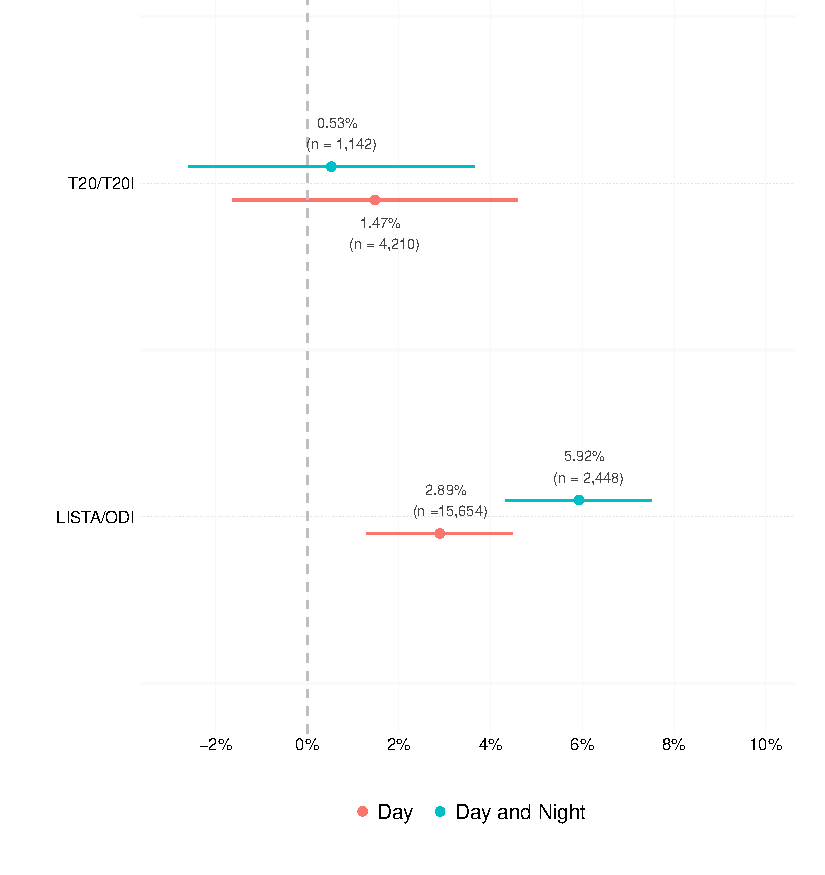
\includegraphics[scale=.85]{../figs/winbyDayNight.pdf}
\label{fig:dn}
\end{figure}

In limited over matches sometimes weather intervenes significantly after the match has already begun. After certain loss of time, the match is generally curtailed and the scores adjusted using a method invented by Duckworth and Lewis \citep[see][]{duckworth1998}. We can use the random nature of who wins the toss to see if winning percentages are strongly conditioned by matches that use Duckworth-Lewis and matches that don't. Again the conventional wisdom suggests that the team that wins the toss is at an advantage in such matches. And again, the conventional wisdom is vindicated. In List A, ODI and domestic Twenty20 matches, the advantage of winning the toss is greater when Duckworth Lewis is used to adjust the scores than when it isn't --- the difference in advantage ranges from about .75\% to over 2\% (see Figure ~\ref{fig:dl}).

\begin{figure}[htbp]
\centering
\caption{Difference in Winning Percentages of Teams that Won the Toss and Teams that Lost the Toss by Whether or not Duckworth-Lewis was invoked}
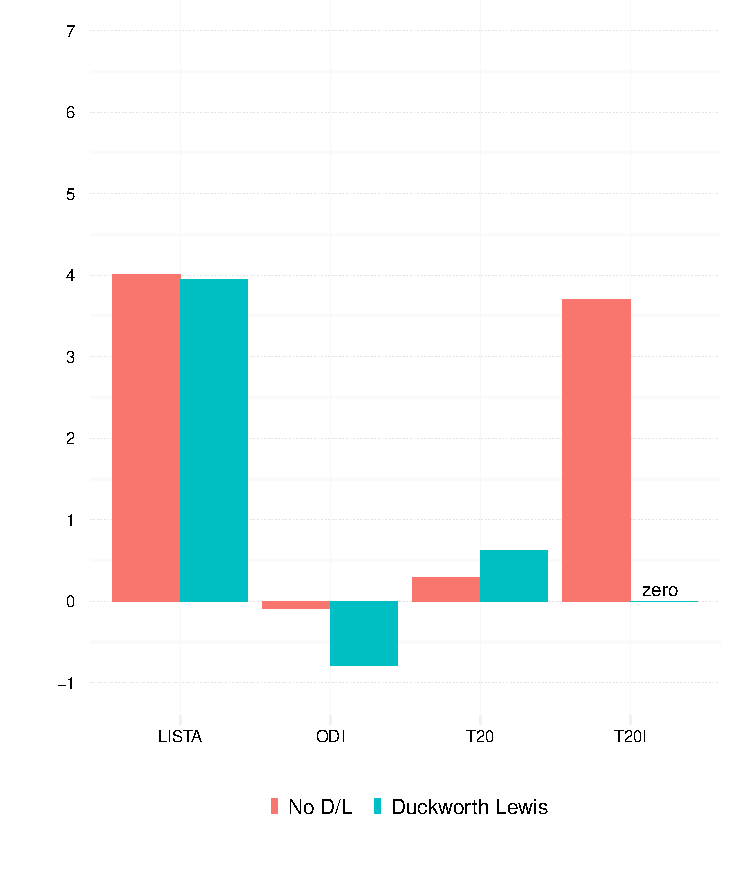
\includegraphics[scale=.85]{../figs/winbyDL.pdf}
\label{fig:dl}
\end{figure}

Winning the toss ought to matter the most when the difference between the quality of the teams that are playing is the least. Similarly, it is unlikely that winning the toss would change who wins the game when two ill-matched teams are playing. To study this, we collected data on team quality. The ICC publishes team ratings for international test and one-day teams each month.\footnote{For details about how the ICC produces these ratings, see \href{http://icc-live.s3.amazonaws.com/cms/media/about_docs/536b1a48c16e5-Reliance\%20ICC\%20ODI\%20Team\%20Rankings\%20FAQs\%202014.pdf}{ICC Rating FAQs}.} Ratings of the ODI teams have been published since 1981, and of test teams, since 1952. Of the entire dataset that spans 1981-today and 1952-today, we only have we have data till 2013.\footnote{The format in which the ICC publishes the ratings changed in 2013. And scraping the latter data posed additional hurdles. We decided that the additional effort wasn't worth the small amount of additional data.} 

Team ratings range from 0 to 143 in our data. For instance, Bangladesh had a rating of 0 in tests for most of 2002 and 2003. And Australia in 2007 twice held a rating of 143. Both seem reasonable. We measure how closely matched the teams by differencing the ranking points of one team from the other. Commercial considerations mean that a majority of the games are played among highly ranked and closely matched teams. So, we limit our analysis to matches where teams ratings differ by no more than 30 points.

The results are expected, but new. As Figure ~\ref{fig:ranks}, there is a sharp curve around 0. When closely matched teams win, the team that wins the toss has a consistent advantage over the team that loses the toss. 

\begin{figure}[htbp]
\centering
\caption{Percentage of Matches Won Minus Matches Lost After Winning the Toss by Difference in Ranks}
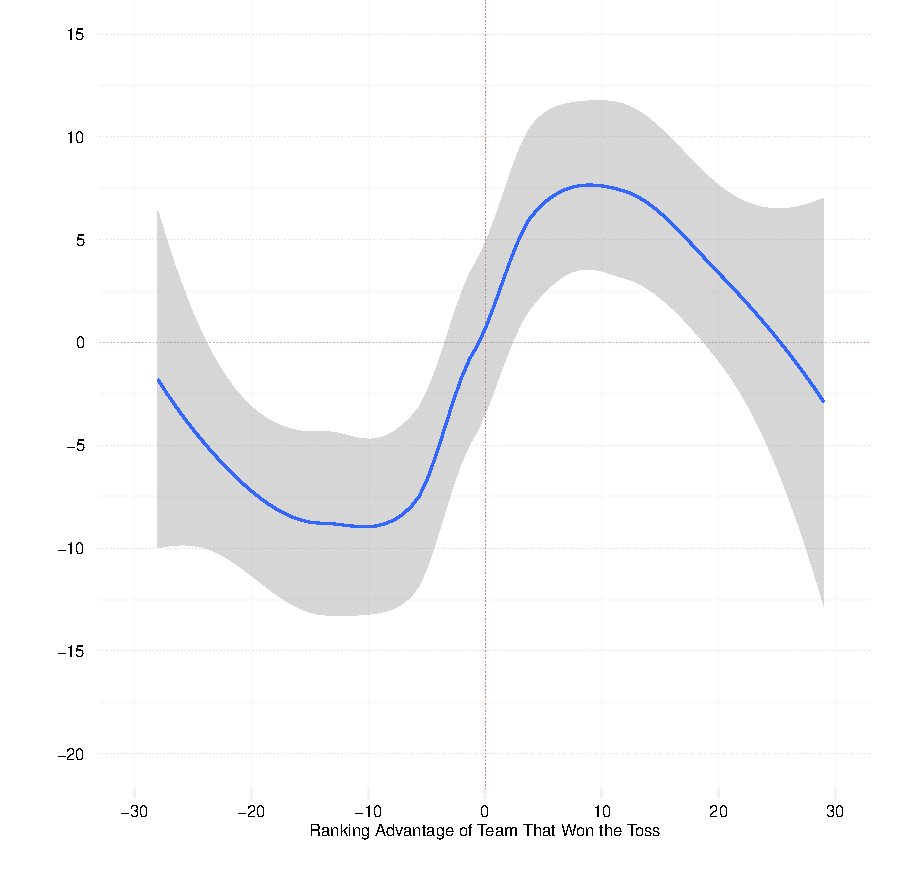
\includegraphics[width=1\textwidth]{../figs/winbyRank.pdf}
\label{fig:ranks}
\end{figure}

How the advantage vary by country? Are some countries better than others? We investigated the question by tallying the advantage by team. Sri Lanka and India do especially well (see ~\ref{fig:country}), coming in at 4.53\% and 3.35\% respectively. Australia and West Indies hover around 1.3--1.5\% and England at 2.33\%. New Zealand, however, does worse when it wins the toss than when it loses it --- difference is about 1.21\%.

\begin{figure}[htbp]
\centering
\caption{Difference in Winning Percentages of Teams that Won the Toss and Teams that Lost the Toss by Country}
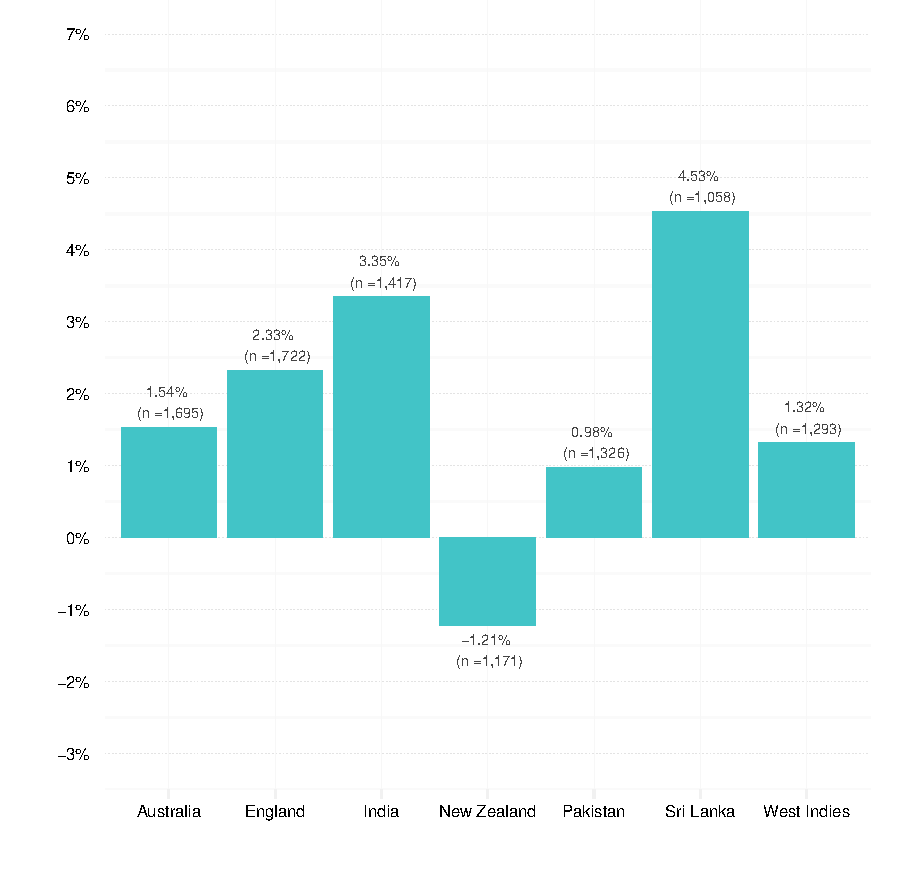
\includegraphics[scale=.85]{../figs/winbyCountry.pdf}
\label{fig:country}
\end{figure}

This isn't a comprehensive inventory of analyses that one could do on the topic. But neither is it meant to be. There are some simple questions that still unanswered. For one, how does the toss advantage vary over time? Have teams become smarter? Other more nuanced but commonly thought questions also remain. For one, students of the game suspect that the advantage of winning a toss in early English season is especially great. We propose to investigate these questions in a follow-up piece.

\clearpage
\bibliographystyle{apsr}
\bibliography{luckybib}

\end{document}